\chapter{Manual de Instalación.}\label{sec:ManualDeInstalacion}

\paragraph{}En este capítulo se va a explicar cómo instalar el entorno de desarrollo
para cada uno de los principales sistemas operativos. Los pasos descritos se podrán
seguir con independencia del estado previo del sistema. No se asume ningún estado previo.

\section{Consideraciones previas}

\paragraph{}El sistema operativo y sus principales tecnologías y herramientas tienen
como base su uso en sistemas operativos GNU/Linux, concretamente la versión 20.04 de
la distribución de Ubuntu. Por lo que, a pesar de poder ser utilizados en cualquier
sistema, serán en éstos donde será más fácil y óptimo su uso.

\paragraph{} Al igual que sucede en otros capítulos de este documento, se van a diferenciar
 las dos partes lógicas que componen el proyecto software.

\section{Instalación del entorno Flutter}

\paragraph{}En el entorno Flutter vamos a ser capaces de desarrollar la aplicación,
pasar sus test y compilarla para diferentes plataformas.

\subsection{Instalación en sistemas operativos GNU/Linux}

\paragraph{}Para la instalación de este entorno en un sistema operativo basado en
la versión de Ubuntu 20.04 se podrá optar por 2 estrategias: correr el entorno de
forma nativa o utilizar el método basado en docker.

\paragraph{Manera nativa:}

\paragraph{}\textbf{Nota:} Este método requiere permisos de \emph{sudo} o super usuario.

\begin{enumerate}
    \item Instalar la herramienta \textbf{\gls{git}} de control de versiones.
    \begin{lstlisting}[style=consola, numbers=left]
        $ sudo apt install git
    \end{lstlisting}

    \item Clonar el repositorio desde github
    \begin{lstlisting}[style=consola, numbers=left]
        $ git clone https://github.com/Gmatarrubia/rpi_weather.git
    \end{lstlisting}

    \item Ejecutar el script de instalación de paquetes.
    \begin{lstlisting}[style=consola, numbers=left]
        $ sudo ./installDevEnv.sh
    \end{lstlisting}

    \item Ejecutar el script de obtención de dependencias.
    \begin{lstlisting}[style=consola, numbers=left]
        $ ./getSources.sh
    \end{lstlisting}

    \item (Opcional) En caso de necesitar instalar Visual Studio Code para el desarrollo,
    podemos utilizar la siguente opctión.
    \begin{lstlisting}[style=consola, numbers=left]
        $ sudo su
        $ source checkFunctions
        $ check_vscode
    \end{lstlisting}

    \item Fin de la instalación.
\end{enumerate}

\paragraph{Entorno de desarrollo dockerizado:}

\paragraph{}\textbf{Nota:} Este método podría requerir permisos de \emph{sudo} o super
usuario.

\begin{enumerate}
    \item Instalar la herramienta \textbf{\gls{git}} de control de versiones.
    \begin{lstlisting}[style=consola, numbers=left]
        $ sudo apt install git
    \end{lstlisting}

    \item Clonar el repositorio desde github
    \begin{lstlisting}[style=consola, numbers=left]
        $ git clone https://github.com/Gmatarrubia/rpi_weather.git
    \end{lstlisting}

    \item Comprobar que el usuario pertenezca al grupo de docker, y en caso que de
    que no pertenezca al grupo, añadirlo.
    \begin{lstlisting}[style=consola, numbers=left]
        $ test $(id | grep -c docker) -eq 0 && sudo usermod -aG $(whoami) docker
    \end{lstlisting}

    \item Ejecutar el script de obtención de dependencias.
    \begin{lstlisting}[style=consola, numbers=left]
        $ ./getSources.sh
    \end{lstlisting}

    \item Fin de la instalación.
\end{enumerate}

\begin{figure}[H]
    \centering
    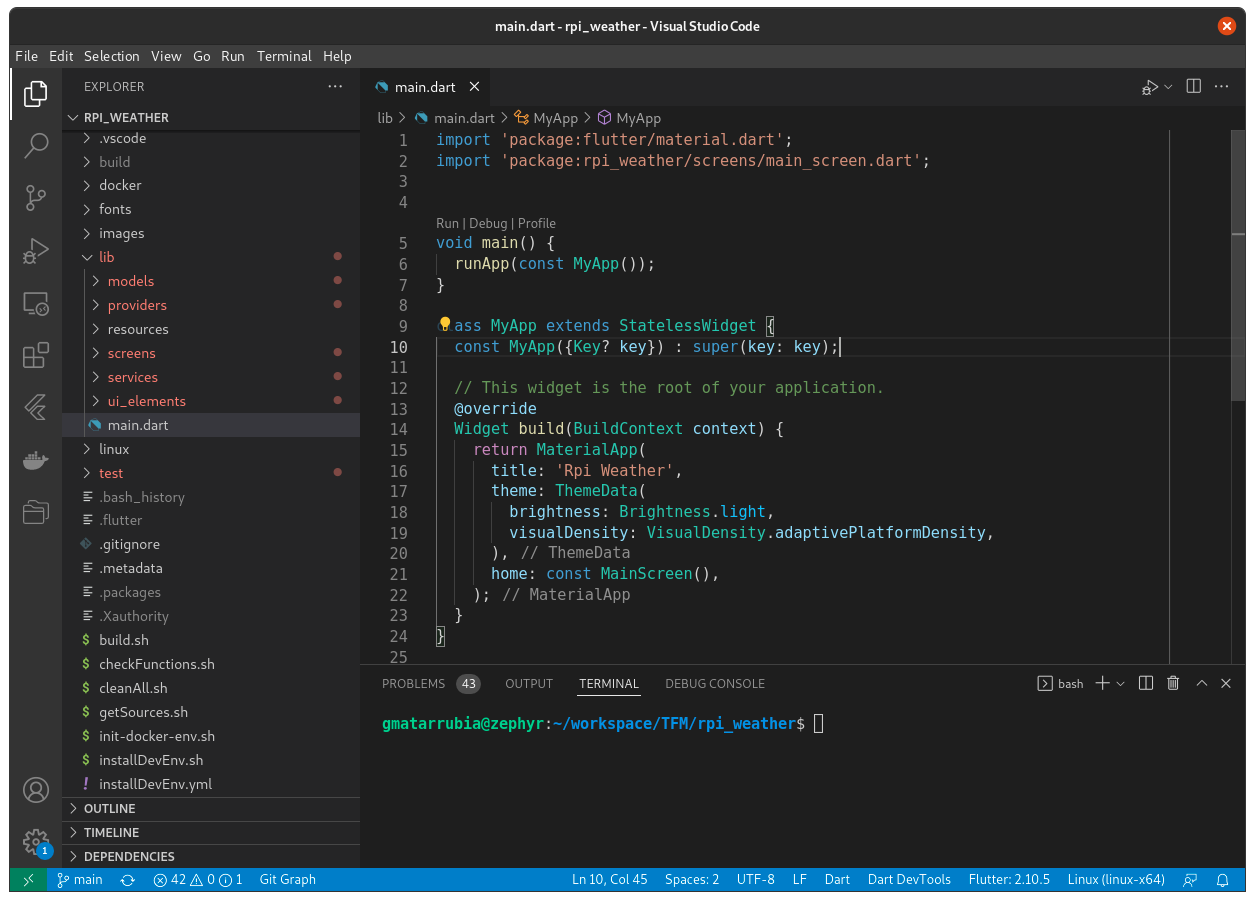
\includegraphics[width=0.95\textwidth]{imgs/vscode-ready}
	\caption[Visual Studio Code]{Visual Studio Code con el proyecto abierto.}
	\label{imgs:vscode-ready}
\end{figure}


\subsection{Instalación en sistemas operativos Windows}

\paragraph{}Blabla

\subsection{Instalación en sistemas operativos MacOS}

\paragraph{}Blabla

\section{Instalación del entorno Yocto}

\subsection{Instalación en sistemas operativos GNU/Linux}

\paragraph{}Blabla

\subsection{Instalación en sistemas operativos Windows}

\paragraph{}Blabla

\subsection{Instalación en sistemas operativos MacOS}

\paragraph{}Blabla

%las referencias a artculos se ponen con \cite,
%las referencias a imgenes \ref,
%las referencias a glosario \gls,
%y las referencias a ecuaciones \eqref